\documentclass{article}

\pdfoutput=1

\usepackage[accepted]{icml2017}
%
% This option will print headings for the title of your paper and
% headings for the authors names, plus a copyright note at the end of
% the first column of the first page.

\usepackage{natbib}
%\usepackage{hyperref}
% use Times
\usepackage{times}
% For figures
\usepackage{graphicx} % more modern
%\usepackage{epsfig} % less modern
\usepackage{subfigure}

\usepackage{tikz}
\usepackage{pgfplots}
\pgfplotsset{filter discard warning=false}

\usepackage{amsmath}
%% \usepackage{amsthm}
%% % \usepackage[english]{babel}
%% \usepackage{tocloft}
\usepackage{color}
%% \usepackage{multirow}
%% % \selectlanguage{english}
\usepackage{algorithm}
\usepackage{algorithmic}
\usepackage{bm}
\usepackage{url}
\usepackage{enumitem}
\usepackage{xspace}

\definecolor{mygreen}{rgb}{0.2, 0.7, 0.2}
\definecolor{myorange}{rgb}{0.9, 0.5, 0.0}

\newcommand\noteMF[1]{\textcolor{red}{MF - #1}}
\newcommand\noteKC[1]{\textcolor{blue}{KC - #1}}
\newcommand\notePM[1]{\textcolor{mygreen}{PM - #1}}
\newcommand\noteSR[1]{\textcolor{myorange}{SR - #1}}

\newcommand{\nobs}{n} % Number of observations
\newcommand{\R}{\mathbb{R}}
\newcommand{\N}{\mathcal{N}}
%\newcommand{\C}{\mathbb{C}}
\newcommand{\Z}{\mathbb{Z}}
\newcommand{\F}{\mathcal{F}}
\newcommand{\I}{\mathcal{I}}
\newcommand{\LL}{\mathcal{L}}
% \newcommand{\vv}{\mathbf{v}}
\newcommand{\uu}{\mathbf{u}}
% \newcommand{\zz}{\mathbf{z}}
% \newcommand{\mm}{\mathbf{m}}
\newcommand{\ee}{\mathbf{e}}

% \newcommand{\KL}{\mathrm{KL}}
% \newcommand{\xnew}{x_{*}}
\newcommand{\xvectnew}{\mathbf{x}_{*}}
% \newcommand{\tildexxnew}{\tilde{\mathbf{x}}_{*}}

%% \newcommand{\T}{\mathrm{T}}
\newcommand{\E}{\mathrm{E}}
\newcommand{\const}{\mathrm{const.}}
\newcommand{\diag}{\mathrm{diag}}
\newcommand{\Tr}{\mathrm{Tr}}
%% \newcommand{\vectorize}{\mathrm{vec}}


\newcommand{\norm}{\mathcal{N}}
%% \newcommand{\expdist}{\mathcal{E}}
%% \newcommand{\DP}{\mathcal{DP}}
%% \newcommand{\Beta}{\mathcal{B}}
%% \newcommand{\Ga}{\mathcal{G}}
%% \newcommand{\Wi}{\mathcal{W}}
%% \newcommand{\St}{\mathrm{St}}
%% \newcommand{\expfam}{\mathcal{E}}

\newcommand{\avect}{\mathbf{a}}
\newcommand{\dvect}{\mathbf{d}}
\newcommand{\fvect}{\mathbf{f}}
\newcommand{\gvect}{\mathbf{g}}
\newcommand{\Ivect}{\mathbf{I}}
\newcommand{\Kvect}{\mathbf{K}}
\newcommand{\hvect}{\mathbf{h}}
\newcommand{\kvect}{\mathbf{k}}
\newcommand{\Lvect}{\mathbf{L}}
\newcommand{\mvect}{\mathbf{m}}
\newcommand{\pvect}{\mathbf{p}}
\newcommand{\svect}{\mathbf{s}}
\newcommand{\uvect}{\mathbf{u}}
\newcommand{\Uvect}{\mathbf{U}}
\newcommand{\vvect}{\mathbf{v}}
\newcommand{\Vvect}{\mathbf{V}}
\newcommand{\zvect}{\mathbf{z}}
\newcommand{\xvect}{\mathbf{x}}
\newcommand{\Xvect}{\mathbf{X}}
\newcommand{\yvect}{\mathbf{y}}
\newcommand{\Yvect}{\mathbf{Y}}
\newcommand{\wvect}{\mathbf{w}}
\newcommand{\Wvect}{\mathbf{W}}
\newcommand{\tvect}{\mathbf{t}}
\newcommand{\zerovect}{\mathbf{0}}
\newcommand{\onesvect}{\mathbf{1}}

\newcommand{\Dobs}{D_\mathrm{obs}}
\newcommand{\Dlat}{D_\mathrm{lat}}

\newcommand{\alphavect}{\boldsymbol{\alpha}}
\newcommand{\betavect}{\boldsymbol{\beta}}
\newcommand{\thetavect}{\boldsymbol{\theta}}
\newcommand{\Thetavect}{\mathbf{\Theta}}
\newcommand{\psivect}{\boldsymbol{\psi}}
\newcommand{\Psivect}{\boldsymbol{\Psi}}
\newcommand{\Phivect}{\boldsymbol{\Phi}}
\newcommand{\Pivect}{\boldsymbol{\Pi}}
\newcommand{\etavect}{\boldsymbol{\eta}}
\newcommand{\rhovect}{\boldsymbol{\rho}}
\newcommand{\tauvect}{\boldsymbol{\tau}}
\newcommand{\nuvect}{\boldsymbol{\nu}}
\newcommand{\muvect}{\boldsymbol{\mu}}
\newcommand{\omegavect}{\boldsymbol{\omega}}
\newcommand{\Omegavect}{\mathbf{\Omega}}
\newcommand{\sigmavect}{\boldsymbol{\sigma}}
\newcommand{\zetavect}{\boldsymbol{\zeta}}
\newcommand{\varepsilonvect}{\boldsymbol{\epsilon}}
\newcommand{\deltavect}{\boldsymbol{\delta}}

\newcommand{\bigO}{\mathcal{O}}


\newcommand{\name}[1]{{\textsc{#1}}\xspace}

\newcommand{\mcmc}{\name{mcmc}}

% DATASETS
% Small
\newcommand{\cifar}{\name{cifar10}}
%% \newcommand{\rectangleshort}{\name{rect-img}}
%% \newcommand{\rectangle}{\name{rectangles-image}}
\newcommand{\mnisteight}{\textsc{mnist}8\textsc{m}\xspace}
%% \newcommand{\mining}{\name{mining}}
\newcommand{\protein}{\name{protein}}
\newcommand{\powerplant}{\name{powerplant}}
\newcommand{\spam}{\name{spam}}
\newcommand{\eeg}{\name{eeg}}
\newcommand{\usps}{\name{usps}}
% Medium
%% \newcommand{\sarcos}{\name{sarcos}} % sarcos all
\newcommand{\mnist}{\name{mnist}} % mnist all
%% \newcommand{\mnistbin}{\name{mnist-b}}
%% \newcommand{\sarcostwo}{\name{sarcos-2}}
% Large
\newcommand{\airline}{\name{airline}}

% Models
\newcommand{\autogp}{\textsc{a}uto\textsc{gp}\xspace}
\newcommand{\gpflow}{\textsc{gpf}low\xspace}
\newcommand{\tensorflow}{\textsc{T}ensor\textsc{F}low\xspace}

\newcommand{\arccosine}{\name{arc-cosine}}
\newcommand{\dbnthree}{\name{DBN}}
\newcommand{\svdkl}{\name{SV-DKL}}
\newcommand{\dgprbf}{\textsc{dgp}-\textsc{rbf}\xspace}
\newcommand{\dgparc}{\textsc{dgp}-\textsc{arc}\xspace}
\newcommand{\dgpep}{\textsc{dgp}-\textsc{ep}\xspace}
\newcommand{\dgpvar}{\textsc{dgp}-\textsc{var}\xspace}

\newcommand{\gplvm}{\name{gplvm}}
\newcommand{\dgplvm}{\name{dgplvm}}
\newcommand{\gp}{\name{gp}}
\newcommand{\gps}{\textsc{gp}s\xspace}
\newcommand{\dgp}{\name{dgp}}
\newcommand{\dgps}{\textsc{dgp}s\xspace}
\newcommand{\dnn}{\name{dnn}}
\newcommand{\dnns}{\textsc{dnn}s\xspace}
\newcommand{\svm}{\name{svm}}
\newcommand{\svms}{\textsc{svm}s\xspace}
\newcommand{\vargp}{\textsc{var}-\textsc{gp}\xspace}

\newcommand{\ard}{\name{ard}}
\newcommand{\softmax}{\name{softmax}}

\newcommand{\relu}{{\textsc{r}}e\name{lu}}

\newcommand{\arc}{\name{arc}}
\newcommand{\rbf}{\name{rbf}}

\newcommand{\adam}{\name{adam}}

% Metrics
\newcommand{\mnll}{\name{mnll}}
\newcommand{\rmse}{\name{rmse}}
\newcommand{\nelbo}{\name{nelbo}}



\newcommand{\mathdefault}[1]{#1}

\linespread{1.2}
% The \icmltitle you define below is probably too long as a header.
% Therefore, a short form for the running title is supplied here:
\icmltitlerunning{Deep Gaussian Processes for Unsupervised Learning}

\newcommand{\quoteauthor}[3]{\begin{quotation} \textit{#1} \end{quotation} \begin{flushright} - #2, \textit{#3}\end{flushright} }


\begin{document}

% If your paper is accepted and the title of your paper is very long,
% the style will print as headings an error message. Use the following
% command to supply a shorter title of your paper so that it can be
% used as headings.
%
%\runningtitle{I use this title instead because the last one was very long}

% If your paper is accepted and the number of authors is large, the
% style will print as headings an error message. Use the following
% command to supply a shorter version of the authors names so that
% they can be used as headings (for example, use only the surnames)
%
%\runningauthor{Surname 1, Surname 2, Surname 3, ...., Surname n}

\twocolumn[
\icmltitle{Deep Gaussian Processes for Unsupervised Learning}

% It is OKAY to include author information, even for blind
% submissions: the style file will automatically remove it for you
% unless you've provided the [accepted] option to the icml2017
% package.

% list of affiliations. the first argument should be a (short)
% identifier you will use later to specify author affiliations
% Academic affiliations should list Department, University, City, Region, Country
% Industry affiliations should list Company, City, Region, Country

% you can specify symbols, otherwise they are numbered in order
% ideally, you should not use this facility. affiliations will be numbered
% in order of appearance and this is the preferred way.
\icmlsetsymbol{equal}{*}

\begin{icmlauthorlist}
\icmlauthor{Simone Rossi}{eurecom}
\icmlauthor{Maurizio Filippone}{eurecom}
\end{icmlauthorlist}

\icmlaffiliation{eurecom}{Department of Data Science, EURECOM, France}

\icmlcorrespondingauthor{Simone Rossi}{rossi@eurecom.fr}
\icmlcorrespondingauthor{Maurizio Filippone}{maurizio.filippone@eurecom.fr}

% You may provide any keywords that you
% find helpful for describing your paper; these are used to populate
% the "keywords" metadata in the PDF but will not be shown in the document
\icmlkeywords{Deep Gaussian Processes, Clustering}

\vskip 0.3in
]

% this must go after the closing bracket ] following \twocolumn[ ...

% This command actually creates the footnote in the first column
% listing the affiliations and the copyright notice.
% The command takes one argument, which is text to display at the start of the footnote.
% The \icmlEqualContribution command is standard text for equal contribution.
% Remove it (just {}) if you do not need this facility.

%\printAffiliationsAndNotice{}  % leave blank if no need to mention equal contribution

\begin{abstract}
Deep Gaussian Processes are modern deep probabilistic models that allow to model complex relationships in observed data. Deep Gaussian Processes are extremely complex to train and we recently made some significant advances in making these scalable. The use of Deep Gaussian Processes has been limited to the case of supervised problems. This project will focus on extending the use of Deep Gaussian Processes to unsupervised problems, notably clustering problems.

TODO
%The composition of multiple Gaussian Processes as a Deep Gaussian Process (\dgp) %enables a deep probabilistic nonparametric approach to flexibly tackle complex %machine learning problems with sound quantification of uncertainty.
%Existing inference approaches for \dgp models have limited scalability and are %notoriously cumbersome to construct.
%In this work we introduce a novel formulation of \dgp{s} based on random feature %expansions that we train using stochastic variational inference.
%This yields a practical learning framework which significantly advances the %state-of-the-art in inference for \dgp{s}, and enables accurate quantification of %uncertainty. % compared to regularized deep neural networks.
%We extensively showcase the scalability and performance of our proposal on several %datasets with up to $8$ million observations, and various \dgp architectures with up %to $30$ hidden layers.
\end{abstract}


\section{Introduction}

The rapid progress of machine learning in the last few years are largely the result of advances in deep learning, combined with the availability of large datasets, fast GPUs and distributed computing solutions (\citet{zoe}). For instance, there are models that can recognize images with an accuracy that rivals that of humans (\citet{dgp}) and this is leading to revolutions in several domains such as autonomous transportation and medical image understanding.


All of these systems, though, currently use \textbf{supervised learning} in which the machine is trained with inputs labeled by humans. The challenge is to let machines learn from raw, unlabeled stream of data. This is known as \textbf{unsupervised learning}; Artificially Intelligent Systems nowadays do not possess ``common sense'', which humans acquire by observing the world, acting in it, and understanding the physical constraints of it. Geo  Hinton, who is a famous professor of ML at the University of Toronto, has said

\quoteauthor{
When we’re learning to see, nobody’s telling us what the right answers are — we just look. Every so often, your mother says “that’s a dog”, but that’s very little information. You’d be lucky if you got a few bits of information — even one bit per second — that way. The brain’s visual system has $10^{14}$  neural connections. And you only live for $10^9$ seconds. So it’s no use learning  one bit per second. You need more like $10^5$ bits per second. And there’s only one place you can get that much information: from the input itself.}{Georey Hinton}{1996 (quoted in (Gorder 2006))}

Two of the most interesting problem concerning unsupervised learning are \textbf{dimensionality reduction} and \textbf{clustering}.

%Approaches to unsupervised learning will be reviewed. This presentation assumes some familiarity with the basic concepts of deep learning.

%Given their impressive performance on machine learning and pattern recognition tasks, Deep Neural Networks (\dnn{s}) have recently attracted a considerable deal of attention in several applied domains such as computer vision and natural language processing; see, e.g., \citet{Lecun15Nature} and references therein.
%Deep Gaussian Processes \citep[\dgp{s};][]{Damianou13} alleviate the outstanding issue characterizing \dnn{s} of having to specify the number of units in hidden layers by implicitly working with infinite representations at each layer.
%From a generative perspective, \dgp{s} transform the inputs using a cascade of Gaussian Processes \citep[\gp{s};][]{Rasmussen06} such that the output of each layer of \gp{s} forms the input to the \gp{s} at the next layer, effectively implementing a deep probabilistic nonparametric model for compositions of functions \citep{Neal96,Duvenaud14}.

%% The flexibility and expressive power of \dgp{s}, however, comes at the expense of having to deal with a model for which learning is extremely difficult.
%Because of their probabilistic formulation, it is natural to approach the learning of \dgp{s} through Bayesian inference techniques; however, the application of such techniques to learn \dgp{s} leads to various forms of intractability.
%A number of contributions have been proposed to recover tractability, extending or building upon the literature on approximate methods for \gp{s}.
%Nevertheless, only few works leverage one of the key features that arguably make \dnn{s} so successful, that is being scalable through the use of mini-batch-based learning \citep{Hensman14,Dai15,Bui16}.
%Even among these works, there does not seem to be an approach that is truly applicable to large-scale problems, and practical beyond only a few hidden layers.

%In this paper, we develop a practical learning framework for \dgp models that significantly improves the state-of-the-art on those aspects.
%In particular, our proposal introduces two sources of approximation to recover tractability, while (i) scaling to large-scale problems, (ii) being able to work with moderately deep architectures, and (iii) being able to accurately quantify uncertainty. % \noteKC{Generalize.}
%The first is a model approximation, whereby the \gp{s} at all layers are approximated using random feature expansions \citep{Rahimi08}; the second approximation relies upon stochastic variational inference to retain a probabilistic and scalable treatment of the approximate \dgp model.

%We show that random feature expansions for \dgp models yield Bayesian \dnn{s} with low-rank weight matrices, and the expansion of different covariance functions results in different \dnn activation functions, namely trigonometric for the Radial Basis Function (\rbf) covariance, and Rectified Linear Unit (\relu) functions for the \arccosine covariance.
%In order to retain a probabilistic treatment of the model % when scaling to large datasets, we employ stochastic variational inference techniques.
%% In particular,
%we adapt the work on variational inference for \dnn{s} and variational autoencoders \citep{Graves11,Kingma14} using mini-batch-based stochastic gradient optimization, which can exploit GPU and distributed computing.
%In this respect, we can view the probabilistic treatment of \dgp{s} approximated through random feature expansions as a means to specify sensible and interpretable priors for probabilistic \dnn{s}.
%Furthermore, unlike popular inducing points-based approximations for \dgp{s}, the resulting learning framework does not involve any matrix decompositions in the size of the number of inducing points, but only matrix products.
%We implement our model in TensorFlow \citep{MartinAbadi15}, which allows us to rely on automatic differentiation to apply stochastic variational inference.




%% This is due to the fact that the nonlinearity introduced by each layer leads to the necessity to solve highly nontrivial integrals which makes it difficult to tractably propagate the uncertainty throughout the layers.
%% ,
%% An additional complication stems from the strong coupling of the \gp{s} at all layers, which are further parameterized by covariance parameters to be optimized or inferred.
% \noteEB{How about the inherent complexity of GPs?}




%% %% An attractive feature of \dgp{s} is that, unlike standard \dnn{s}, their probabilistic formulation allows for a principled way to tackle quantification of uncertainty and model selection, which is desirable when employing deep models in practice. % \noteKC{To be cleared up}
%% %% \noteEB{But so do Bayesian DNNs, unclear why DGPs are different here}

%% %% While approximations have been developed to recover tractability in general Bayesian inference tasks \citep{Candela05,Titsias09,Hensman15,Dezfouli15}, their application to \dgp{s} remains nonetheless challenging.



%% %% Although our approach is amenable to any stationary covariance function, we develop it in detail for the squared exponential and arc-cosine covariance functions.
%% Applying random feature expansions to \dgp{s}, we obtain \dnn{s} with low-rank weight matrices.
%% Feature expansions of different covariance functions result in different \dnn activation functions, namely trigonometric for the radial basis function covariance, and rectified linear unit functions for the arc-cosine covariance.
%% By virtue of the connection to \dnn{s}, we are able to employ scalable optimization and inference techniques that have been developed in the literature to train \dnn{s}, allowing the proposed \dgp model to scale to large data in the same way as \dnn{s}.

%% In order to retain a probabilistic treatment of the model when scaling to large datasets, we employ stochastic variational inference techniques.
%% In particular, we adapt the work on variational inference for \dnn{s} and variational autoencoders \citep{Graves11,Kingma14,Rezende14} using mini-batch-based stochastic gradient optimization for the proposed \dgp model, which can exploit GPU and distributed computing.
%% We implement the model in TensorFlow \citep{MartinAbadi15}, which allows us to rely on automatic differentiation during the optimization procedure.
%% %% The impact of the variational approximation, as opposed to characterizing the full posterior distribution over all model parameters, is the most difficult to assess.
%% In the supplementary material, we also illustrate the quality of our approximation by comparing the variational approximation of the proposed model with % a run of a
%% the inference resulting from the application of Markov chain Monte Carlo (\mcmc) methods that we develop for two-layer \dgp regression models.

%Although having to select the appropriate number of random features goes against the nonparametric formulation favored in \gp models, the level of approximation can be tuned based on constraints on running time or hardware.
%Most importantly, the random feature approximation enables us to develop a learning framework for \dgp{s} which significantly advances the state-of-the-art.
%We extensively demonstrate the effectiveness of our proposal on a variety of regression and classification problems by comparing it with \dnn{s} and other state-of-the-art approaches to infer \dgp{s}.
%The results indicate that for a given \dgp architecture, our proposal is consistently faster at achieving lower errors compared to the competitors.
%Another key observation is that the proposed \dgp outperforms \dnn{s} trained with dropout on quantification of uncertainty metrics.

%We focus part of the experiments on large-scale problems, such as \mnisteight digit classification and the \airline dataset, which contain over $8$ and $5$ million observations, respectively.
%Only very recently there have been attempts to demonstrate performance of \gp models on such large data sets \citep{Wilson16,Krauth17}, and our proposal is on par with these latest \gp methods.
%Furthermore, we obtain impressive results when employing our learning framework to \dgp{s} with moderate depth (few tens of layers) on the \airline dataset.
%We are not aware of any other \dgp models having such depth that can achieve comparable performance when applied to datasets with millions of observations.
%Crucially, we obtain all these results by running our algorithm on a single machine without GPUs, but our proposal is designed to be able to exploit GPU and distributed computing to significantly accelerate our deep probabilistic learning framework (see supplement for experiments in distributed mode). % ; for completeness we also report some prelimiary results on the performance of an asynchronous distributed version of our code in the supplementary material.

%% Such an undertaking would not have been computationally feasible using a regular \gp model, while other \dgp approaches do not converge as quickly as our technique.

% \noteMF{Change - Furthermore, the inclusion of an asynchronous implementation of stochastic gradient optimization allows us to exploit large-scale computing facilities using distributed updates, showing that we can truly scale \dgp{s} to tractably tackle unprecedently large amounts of data.} \noteKC{Now moved to supplementary.}% \notePM{To be discussed, but I'd be careful here. Even the mnsit 8M is not that big, so we cannot really claim we learn from big data. What we do is that we exploit parallelism to lower training time, provided that our experiments really show this.}

%In summary, the most significant contributions of this work are as follows:
%% \begin{itemize}
%% \item
%(i) we propose a novel approximation of \dgp{s} based on random feature expansions that we study in connection with \dnn{s};
%(ii) we demonstrate the ability of our proposal to systematically outperform state-of-the-art methods to carry out inference in \dgp models, especially for large-scale problems and moderately deep architectures;
%(iii) we validate the superior quantification of uncertainty offered by \dgp{s} compared to \dnn{s}.

%% \noteEB{May be we can focus on why DGPs are good. Flexible (non-parametric) approaches to quantifying uncertainty in DNNs. By using random features, we have a state-of-the-art way to train these models. While the resulting model is a Bayesian DNNs, we still mantain the theoretical connection with DGPs, which is important for prior setting, variable initialization and posterior analysis. In fact, we do use these tree advantages in our experiments!}

%% The paper is organized as follows.
%% The rest of this section reports the related work.
%% Sec.~2 introduces \dgp{s} and demonstrates how covariance functions can be approximated with random features.
%% In Sec.~3, we propose our construction of \dgp{s} using such approximations, and show how the resulting model can be learned using stochastic variational inference.
%% Sec.~4 reports an extensive evaluation of our proposal and a thorough comparison with state-of-the-art approaches to learn \dgp{s} and \dnn{s}, while Sec.~5 concludes the paper.
%% \noteEB{No one really reads the paragraph above, we can get rid of it and make some room.}

\subsection{Related work}

TODO 
%Following the original proposal of \dgp models in \citet{Damianou13}, there have been several attempts to extend \gp inference techniques to \dgp{s}.Notable examples include the extension of inducing point approximations \citep{Hensman14,Dai15} and Expectation Propagation \citep{Bui16}. Sequential inference for training \dgp{s} has also been investigated in \citet{Wang16}. A recent example of a \dgp ``natively'' formulated as a variational model appears in \citet{Tran16}. Our work is the first to employ random feature expansions to approximate \dgp{s} as \dnn{s}. The expansion of the squared exponential covariance for \dgp{s} leads to trigonometric \dnn{s}, whose properties were studied in \citet{Sopena99}. Meanwhile, the expansion of the arc-cosine covariance is inspired by \citet{Cho14}, and it allows us to show that \dgp{s} with such covariance can be approximated with \dnn{s} having \relu activations.

%The connection between \dgp{s} and \dnn{s} has been pointed out in several papers, such as \citet{Neal96} and \citet{Duvenaud14}, where pathologies with deep nets are investigated. The approximate \dgp model described in our work becomes a \dnn with low-rank weight matrices, which have been used in, e.g., \citet{Novikov15,Sainath13,Denil13} as a regularization mechanism. Dropout is another technique to speed-up training and improve generalization of \dnn{s} that has recently been linked to variational inference \citep{Gal16}.

%Random Fourier features for large scale kernel machines were proposed in \citet{Rahimi08}, and their application to \gp{s} appears in \citet{Gredilla10}. In the case of squared exponential covariances, variational learning of the posterior over the frequencies was proposed in \citet{Gal15} to avoid potential overfitting caused by optimizing these variables. These approaches are special cases of our \dgp model when using no hidden layers.

%In our work, we learn the proposed approximate \dgp model using stochastic variational inference. Variational learning for \dnn{s} was first proposed in \citet{Graves11}, and later extended to include the reparameterization trick to clamp randomness in the computation of the gradient with respect to the posterior over the weights \citep{Kingma14,Rezende14}, and to include a Gaussian mixture prior over the weights \citep{Blundell15}.


% \mcmc inference of Bayesian \dnn{s} was studied in \citet{Neal96}. --> not needed
% We adapt the Elliptical Slice Sampling algorithm in \citet{Murray10b} to obtain an \mcmc sampler for a two-layer \dgp model with Gaussian likelihood.

%!TEX root = report.tex

\section{Preliminaries}

This section will be dedicated to review the main idea behind Gaussian Processes (\gp) and a possible deep architecture built on top of them (\dgp).

\subsection{Gaussian Process}

A Gaussian process (\gp) is a generalization of the Gaussian probability distribution: whereas a probability distribution describes random variables which are scalars or vectors (for multivariate distributions), a stochastic process governs the properties of functions. Even though there are two different perspectives for looking at a \gp, for the following formulation of the \dgp, here it's present only the weight-space view.

The weight-space representation of \gp for regression is the natural extension of the Bayesian linear regression, where the the number of features for each sample is potentially infinite. Consider a supervised learning problem where a set of input vectors $\Xvect = [\xvect_1, \ldots, \xvect_\nobs]^{\top}$ is associated with a set of labels $Y = [y_1, \ldots, y\nobs]^{\top}$, where $\xvect_i \in R^{D_{\mathrm{in}}}$ and $y_i \in R$.

Stating from the input $X$, the design matrix $\Phivect$ can be computed applying a set of potentially non linear basis functions. Specifically, we introduce the function $\phi(\xvect)$ which maps a $D_{in}$-dimensional input vector x into an $F$  dimensional feature space as follow:
\begin{equation}
    \Phi_i = \phi(\xvect_i) \quad \mbox{with} \quad \phi:R^{D_{\mathrm{in}}}    \rightarrow R^F
\end{equation}

As long as the projections are fixed functions and independent on the parameters, the model is still linear in the parameters, and therefore analytically tractable.

Without entering into details, it can be proved that, for both training and prediction, the model is defined exclusively in terms of inner products in the input space that can be lifted into feature space by replacing occurrences of those product with a function $k(\xvect_0, \xvect_1)$, such that:

\begin{equation}
    k(\xvect_0, \xvect_1) = \phi(\xvect_0)^\top\phi(\xvect_1)
\end{equation}

This technique is particularly useful in situations where it is more convenient to compute the kernel than the feature vectors themselves. Moreover, since both in training and in prediction matrix inversion (which computational cost is $\bigO(n^3)$) are involved, when the number of features starts increasing, it's more convenient to invert a $\nobs\times\nobs$ matrix than a $F\times F$ one. In addition to that, since kernel functions can be computed without building the feature vectors and the mapping function $\phi$, it's also possible to infer an infinite feature space dimension while keeping all the computations feasible.

One of the most famous kernels, also called covariance function, that embeds an infinite feature space dimension is the Radial Basis Function (\rbf), defined as follows

\begin{equation} \label{eq:covariance:rbf:ard}
k_{\mathrm{rbf}}(\xvect, \xvect^{\prime}) =
\exp\left[-\frac{1}{2} \left\| \xvect - \xvect^{\prime} \right\|^{\top}  \right]
\end{equation}

It will be used in the following treatise as starting point for making \gp{s} scalable in a deep architecture.

\subsection{Deep Gaussian Processes}


%\input{figures/diagram.tex}
In this work, we build the deep architecture following the model firstly introduced by \citet{Filippone2017}. Generally, in deep models, the mapping between inputs and labels is expressed as a composition of functions
\begin{equation}
\fvect(\xvect) = \left(\fvect^{(N_{\mathrm{h}} - 1)} \circ \ldots \circ \fvect^{(0)}\right)(\xvect),
\end{equation}
where, in this case, each of the $N_{\mathrm{h}}$ layers is finite set of \gp{s}.

In contrast to Deep Neural Networks (\dnn{s}), where each of the hidden layers implements a parametric function of its inputs, in \dgp{s} these functions are assigned a \gp prior, and are therefore nonparametric.

\subsubsection{Random Fourier Expansion}

With reference to the Bochner's theorem, any continuous covariance function $k(\xvect_i, \xvect_j) = k(\xvect_i - \xvect_j)$ is positive definite if and only if it can be rewritten as the Fourier transform of a non-negative measure $p(\omegavect)$. Denoting the spectral frequencies by $\omegavect$, in the case of the \rbf covariance in equation~\ref{eq:covariance:rbf:ard}, this yields:

\begin{equation}
k_{\mathrm{rbf}}(\xvect_i - \xvect_j) = \int p(\omegavect) \exp\left[i (\xvect_i - \xvect_j)^{\top} \omegavect \right] d\omegavect \text{.}
\end{equation}

Because the covariance function and the non-negative measures are real, we can drop the unnecessary complex part of the argument of the expectation, keeping $\cos((\xvect_i - \xvect_j)^{\top} \omegavect)$ that can be rewritten as
$\cos(\xvect_i^{\top} \omegavect) \cos(\xvect_j^{\top} \omegavect) + \sin(\xvect_i^{\top} \omegavect) \sin(\xvect_j^{\top} \omegavect)$.
% Note that an alternative representation using only cosines can be found by introducing a uniformly distributed phase term \citep{Rahimi08,Gal16}.

The importance of the expansion above is that it allows us to interpret the covariance function as an expectation that can be estimated using Monte Carlo.
Defining $\zvect(\xvect | \omegavect) = [\cos(\xvect^{\top} \omegavect), \sin(\xvect^{\top} \omegavect)]^{\top}$,
the covariance function can be therefore unbisedly approximated as % by the following (unbiased) Monte Carlo estimate
\begin{equation}
%% k_{\mathrm{rbf}}(\xvect_i, \xvect_j | \thetavect) \approx \frac{\sigma^2}{N_{\mathrm{RF}}} \sum_{r=1}^{N_{\mathrm{RF}}} \zvect(\xvect_i | \tilde{\omegavect}_r)^{\top} \zvect(\xvect_j | \tilde{\omegavect}_r) \text{,}
k_{\mathrm{rbf}}(\xvect_i, \xvect_j) \approx \frac{1}{N_{\mathrm{RF}}} \sum_{r=1}^{N_{\mathrm{RF}}} \zvect(\xvect_i | \tilde{\omegavect}_r)^{\top} \zvect(\xvect_j | \tilde{\omegavect}_r) \text{,}
\end{equation}
with $\tilde{\omegavect}_{r} \sim p(\omegavect)$.
%% In practice, this expansion leads to an explicit representation of the mapping induced by the choice of covariance function.
This has an important practical implication, as it provides the means to access an approximate explicit representation of the mapping induced by the covariance function that, in the \rbf case, we know is infinite dimensional.

\subsubsection{Deep Architecture}

With reference to \citet{Filippone2017} work, the architecture that will be used as starting point for the analysis of the unsupervised case is represented in Figure \ref{fig:DGP:diagram}.

\input{figures/diagram.tex}

Considering a \dgp with \rbf covariances, using the aforementioned expension, we have that
\begin{equation}
\Phi_{\mathrm{rbf}}^{(l)} = \sqrt{\frac{(\sigma^2)^{(l)}}{N_{\mathrm{RF}}^{(l)}}} \left[ \cos\left(F^{(l)} \Omega^{(l)}\right), \sin\left(F^{(l)} \Omega^{(l)}\right) \right] \text{,}
\end{equation}
and
%% \begin{equation}
$
F^{(l+1)} = \Phi_{\mathrm{rbf}}^{(l)} W^{(l)} % \text{.}
$.

%!TEX root = report.tex

\section{Deep models for dimensionality reduction}
One of the most important problems in unsupervised learning is to represent the observed data $\Yvect$ (with $\yvect_i \in R^{D_\mathrm{obs}}$) in some lower dimensional embedded space $\Xvect$ (with $\xvect_i \in R^{D_\mathrm{lat}}$). In a probabilistic model, the $\Xvect$ space is also known as \emph{latent space}, while all the variables $\xvect_i \in \Xvect$ are called \emph{latent variables}.

In the last decades, a lot of effort has been put in action for building the ``optimal'' mapping function between $R^{\Dobs}$ and $R^{\Dlat}$ (see, for instance, \noteSR{Put references to PCA and Kernel PCA}). In the next sections, we will review the key idea of Latent Variable Model and its natural extension to \gplvm.

\subsection{Dual Probabilistic PCA}
Typically, in the context of dimensionality reduction, we specify a latent variable model that relate a set of latent variables $\Xvect \in R^{\nobs\times \Dlat}$ to a set of observed variables $\Yvect \in R^{\nobs\times \Dobs}$, through a set of potentially non linear parameters. The model is defined probabilistically, the latent variables are marginalized and the parameters are maximized.

\citet{Lawrence2005} proved that, for a particular choice of Gaussian likelihood, this is the same as marginalize the parameters and maximize the latent variables. Moreover, it can be proved that for a particular choice of prior distribution on the parameters, this probabilistic model is equivalent to the probabilistic PCA \citep{Bishop1999}.

Let's start by specifying a prior for $\Wvect$ and let it be a simple spherical Gaussian distribution:

\begin{equation}
    p(\Wvect) = \prod_{i=0}^{\Dobs-1}\N(\wvect_i\vert\zerovect, \Ivect)
\end{equation}

The corresponding log-likelihood is

\begin{equation}
    \label{eq:likelihood:lvm:lawrence}
    \log p(\Yvect\vert\Xvect,\sigma^2) =  - \dfrac{\Dobs}{2}\ln\vert\Kvect\vert - \dfrac{1}{2}\Tr\left(\Kvect^{-1}\Yvect\Yvect^\top\right) + \alpha\text{,}
\end{equation}

where $\Kvect = \Xvect\Xvect^\top + \sigma^2\Ivect$ and $\alpha = -\tfrac{\nobs\Dobs}{2}\ln(2\pi)$ is normalization constant independent with the latents.

\citet{Lawrence2005} proved that the maximization of the likelihood in Equation \ref{eq:likelihood:lvm:lawrence} with respect to the latent variables $\Xvect$ turns out to be the solution of the eigenvalue problem of the classic PCA.

If fact, the solution of this optimization problem can be written in closed form as it follows

\begin{equation}
    \label{eq:ppca:latent:solution}
    \Xvect = \Uvect\Lvect\Vvect^\top
\end{equation}

where $\Uvect$ is an $\nobs\times\Dlat$ matrix whose columns are the first $\Dlat$ eigenvectors of $\Yvect\Yvect^\top$, $\Lvect$ is the associated diagonal eigenvalue matrix and $\Vvect$ is eventually a $\Dobs\times\Dobs$ rotation matrix.

\subsection{Gaussian process latent variable model}

From the analysis of Equation (\ref{eq:likelihood:lvm:lawrence}), we can immediately see that the marginal likelihood for dual probabilistic PCA is a product of $\Dobs$ independent Gaussian processes with linear covariance function.

What will be done next is to replace the inner product kernel with a covariance function so that it allows non-linear functions to obtain a non-linear latent variable model. Due to the close relationship with the linear model, which has an interpretation as probabilistic PCA, such a model can be interpreted as a non-linear probabilistic version of PCA or, as it will be referred to, Gaussian process latent variable model (or \gplvm).

Unfortunately, though, in general there is not closed form solution of the maximization of the likelihood and therefore the
resulting models will not be optimizable through an eigenvalue problem. The covariance function that will be used in the following examples is the Squared Exponential in Equation (\ref{eq:covariance:rbf:ard}). As result, the log-likelihood is a highly non-linear function of the latents and the parameters. We are therefore forced to use automatic optimisation tools, such as the stochastic gradients and \adam optimizer \citep{Kingma2015} already implemented in \tensorflow.

\subsubsection{Extension to deep models}

In the previous sections, we showed how the problem of dimensionality reduction can be connected to a \gplvm. Now, we will show that, without great changes in the formulation, this model can be extended to \dgplvm. This is justified by the fact that when the functional relationship between variables is non-stationary, traditional \gp{s} fail, while \dgp can better adapt to handle non-stationary functions.

In the \dgplvm, the likelihood associated to the model is optimized using variational inference. Let $p(\Yvect\vert\Xvect,\Xi)$ the likelihood of the model, where $\Xi$ is the set of all parameters. As proved by \citet{Filippone2017}, defining $\LL$ the log-likelihood and $\mathcal{E} = \E_{q(\Wvect)} \left( \log\left[ p\left(\Yvect | \Xvect, \Wvect, \Xi\right) \right] \right)$, we obtain

\begin{equation}
\LL \geq \mathcal{E}
%% \E_{q(\Wvect)} \left( \log\left[ p\left(Y | X, \Wvect, \Omegavect, \Thetavect\right) \right] \right)
- \mathrm{DKL}\left[q(\Wvect) \| p\left(\Wvect\right)\right] \text{,}
\end{equation}
where $q(\Wvect)$ acts as an approximation to the posterior over all the weights $p(\Wvect | \Yvect, \Xvect, \Xi)$.

Optimizing the variational lower bound with respect to $q(\Wvect)$ and to $\Xvect$, we will obtain a model equivalent to a deep Gaussian process latent variable model (or, as it will be referred to, \dgplvm).

%!TEX root = report.tex

\section{Deep models for clustering}

The second classical problem of unsupervised learning is clustering. \noteSR{Add something general on clustering}

\subsection{Extended \dgplvm}

The architecture already discussed in the previous sections can be also adapted to handle clustering assignment.

Our intent is to build a probabilistic model, such that for each observation $\yvect_i$ it gives a probability of being assigned to a cluster; formally we want to compute

\begin{equation}
    \tilde k = \arg\max_{k}p(x_{ij}=k\vert\yvect_i, \Xi)
\end{equation}

where $\Xi$ is the set of all the parameters and hyper-parameters of the model. This can be connected do a latent variable model, since the vector of label probability $\xvect_i$ is an hidden variable and it's never observed in the training set.

This is achieved keeping the same architecture presented in Figure \ref{fig:DGP:diagram} and replacing the first layer of \gp{s} with a \softmax layer. The \softmax layer simply implements a softmax function on each samples of the latent space $\Xvect$; in practice:

\begin{equation}
    \Pivect = \dfrac{\exp(\Xvect)} {\sum_{j=0}^{D\mathrm{lat} - 1} \exp(\Xvect_{:,j})}
\end{equation}

where $\Pivect$ is a $\nobs\times\Dlat$ matrix of probabilities and $\Dlat$ is the number of cluster imposed to the model.

\def\layersep{1.8cm}
\def\scale{0.5}
\definecolor{myblue}{rgb}{0.2, 0.2, 0.8}
\newcommand{\red}{\textcolor{red}}
\newcommand{\orange}{\textcolor{orange}}
\newcommand{\green}{\textcolor{green}}
\newcommand{\blue}{\textcolor{blue}}
\newcommand\colorpar[1]{\textcolor{myyellow}{#1}}
\newcommand\colordata[1]{\textcolor{myorange}{#1}}
\newcommand\colorlatent[1]{\textcolor{myblue}{#1}}
\newcommand\colorweights[1]{\textcolor{mygreen}{#1}}

\begin{figure}[t]
\begin{tikzpicture}[shorten >=1pt,->,draw=green!50!black, node distance=\layersep]
    \tikzstyle{every pin edge}=[<-,shorten <=1pt]
    \tikzstyle{neuron}=[circle,minimum size=10pt,inner sep=0pt, draw=black]

    \tikzstyle{data neuron}=[neuron, fill=yellow!50!red];
    \tikzstyle{output neuron}=[neuron, fill=blue!50];
    \tikzstyle{hidden neuron}=[neuron];
    \tikzstyle{annot} = [text width=4em, text centered];
    \tikzstyle{annot-weight} = [text centered, fill=white!20, rectangle, draw];

    %% % Draw the input layer nodes
    %% \foreach \name / \y in {1,...,4}
    %%     \node[data neuron, pin=left:{\scriptsize $X$ \#\y}] (F0-\name) at (0,-\y) {};

    % Draw the input layer nodes
    \foreach \name / \y in {1,...,4}
        \node[data neuron] (F0-\name) at (0,\scale*-\y) {};

    % Draw the first hidden layer nodes - Phi^{(0)}
    %\foreach \name / \y in {1,...,5}
    %    \path[yshift=\scale*0.5cm]
    %        node[hidden neuron] (Phi0-\name) at (\layersep,\scale*-\y cm) {};

    % Draw the layer node for F^{(1)}
    \foreach \name / \y in {1,...,4}
        \path[yshift=\scale]
            node[output neuron] (F1-\name) at (1 * \layersep,\scale*-\y) {};

    % Draw the second hidden layer nodes - Phi^{(1)}
    \foreach \name / \y in {1,...,5}
        \path[yshift=\scale*0.5cm]
            node[hidden neuron] (Phi1-\name) at (2 * \layersep,\scale*-\y cm) {};

    % Draw the layer node for F^{(1)}
    \foreach \name / \y in {1,...,3}
        \path[yshift=\scale*-0.5cm]
            node[output neuron] (F2-\name) at (3 * \layersep,\scale*-\y) {};

    \foreach \name / \y in {1,...,3}
        \path[yshift=\scale*-0.5cm]
            node[data neuron] (Y-\name) at (4 * \layersep,\scale*-\y) {};

    % Draw Thetas
    %\node[annot] (theta-0) at (0.5 * \layersep,\scale*-4.5) {\scriptsize\red{$\thetavect$}$^{(0)}$};
    %\node[annot] (theta-1) at (2.5 * \layersep,\scale*-4.5) {\scriptsize\red{$\thetavect$}$^{(1)}$};


    %% \node[output neuron,pin={[pin edge={->}]right:{\scriptsize $F^{(1)}$}}, right of=Phi1-3] (F2) {};


    % Connect every node in the input layer with every node in the
    % hidden layer.
    %\foreach \source in {1,...,4}
    %    \foreach \dest in {1,...,5}
    %        \path (F0-\source) edge (Phi0-\dest);

    % Connect every node in the hidden layer with the output layer
    \foreach \source in {1,...,4}
        \foreach \dest in {1,...,4}
            \path (F0-\source) edge (F1-\dest);

    % Connect every node in the hidden layer with the output layer
    \foreach \source in {1,...,4}
        \foreach \dest in {1,...,5}
            \path (F1-\source) edge (Phi1-\dest);

    % Connect every node in the hidden layer with the output layer
    \foreach \source in {1,...,5}
        \foreach \dest in {1,...,3}
            \path (Phi1-\source) edge (F2-\dest);

    % Connect every node in the hidden layer with the output layer
    \foreach \source in {1,...,3}
        \foreach \dest in {1,...,3}
            \path (F2-\source) edge (Y-\dest);

    % Annotate the layers
    \node[annot,above of=Phi0-1, node distance=0.6cm] (Layer-Phi0) {{\scriptsize $\colorlatent{\Pivect}$}};
    \node[annot,left of=Layer-Phi0] {{\scriptsize $\colordata{X}$}};
    %\node[annot,right of=Layer-Phi0] {{\scriptsize $\colorlatent{\Pivect}$}};
    \node[annot,above of=Phi1-1, node distance=0.6cm] (Layer-Phi1) {{\scriptsize $\Phi^{(1)}$}};
    \node[annot,right of=Layer-Phi1] (Layer-F2) {{\scriptsize $\colorlatent{F}^{(2)}$}};
    \node[annot,right of=Layer-F2] (Layer-Y) {{\scriptsize $\colordata{Y}$}};


    \node[annot-weight] (Omega-Phi0) at (0.5 * \layersep, \scale*-2.5) {{\scriptsize $\colorweights{\softmax}$}};
    %\node[annot-weight,right of=Omega-Phi0] (W-Phi0) {{\scriptsize $\colorweights{W}^{(0)}$}};
    \node[annot-weight] (Omega-Phi1) at (1.5 * \layersep, \scale*-2.5) {{\scriptsize $\colorweights{\Omega}^{(1)}$}};
    \node[annot-weight,right of=Omega-Phi1] (W-Phi1) {{\scriptsize $\colorweights{W}^{(1)}$}};

    %\path (theta-0) edge[red] (Omega-Phi0);
    %\path (theta-1) edge[red] (Omega-Phi1);

\end{tikzpicture}
\label{fig:DGP:diagram}
\end{figure}

Invariance to rotations and to initialisation

Probabilistic model

%!TEX root = report.tex

\section{Experiments}

TODO

\subsection{Dimensionality reduction for visualisation}

TODO

\subsubsection{Latents initialization}

TODO

\subsection{Clustering}

TODO

%\section{Conclusions}

In this work, we have proposed a novel formulation of \dgp{s} which exploits the approximation of covariance functions using random features, as well as stochastic variational inference for preserving the probabilistic representation of a regular \gp.
We demonstrated how inference using this model is not only faster, but also frequently superior to other state-of-the-art methods, with particular emphasis on competing \dgp models.
The results obtained for both the \airline dataset and the \mnisteight digit recognition problem are particularly impressive since such large datasets have been generally considered to be beyond the computational scope of \dgp{s}.
We perceive this to be a considerable step forward in the direction of scaling and accelerating \dgp{s}.

The results obtained on higher-dimensional datasets strongly suggest that approximations such as Fastfood~\cite{Smola13} could be instrumental in the interest of using more random features.
We are also currently investigating ways to mitigate the decline in performance observed when optimizing $\Omegavect$ variationally with resampling. 
The obtained results also encourage the extension of our model to include residual learning or convolutional layers suitable for computer vision applications.

%\subsubsection*{Acknowledgements}

MF gratefully acknowledges support from the AXA Research Fund.


\bibliography{report}
\bibliographystyle{icml2017}

%\appendix 
\onecolumn
%\icmltitle{Supplementary Material \\ Random Feature Expansions for Deep Gaussian Processes}

\section{Additional Experiments}

Using the experimental set-up described in Section 4, Figure~\ref{fig:mnll_vs_time} demonstrates how the competing models perform with regards to the \rmse (or error rate) and \mnll metric when two hidden layers are incorporated into the competing models.
The results follow a similar progression to those reported in Figure~3 of the main paper.
The \dgparc and \dgprbf models both continue to perform well after introducing this additional layer.
However, the results for the regularized \dnn are notably inferior, and the degree of overfitting is also much greater.
To this end, the \mnll obtained for the \mnist dataset is not shown in the plot as it was vastly inferior to the values obtained using the other methods.
\dgpep was also observed to have low scalability in this regard whereby it was not possible to obtain sensible results for the \mnist dataset using this configuration.
 
\input{figures/comparison_3l}

In Section 3.3, we outlined the different strategies for treating $\Omegavect$, namely fixing them or treating them variationally, where we observed that the constructed \dgp model appears to work best when these are treated variationally while fixing the randomness in their computation throughout the learning process (\name{var-fixed}).
In Figures~\ref{fig:optim_error} and~\ref{fig:optim_mnll}, we compare these three approaches on the complete set of datasets reported in the main experiments for one and two hidden layers, respectively.
Once again, we confirm that the performance obtained using the \name{var-fixed} strategy yields more consistent results than the alternatives.
This is especially pertinent to the classification datasets, where the obtained error rate is markedly superior.
However, the variation of the model constructed with the \arccosine kernel and optimized using \name{var-fixed} appears to be susceptible to some overfitting for higher dimensional datasets (\spam and \mnist), which is expected given that we are optimizing several covariance parameters (\ard).
This would motivate trying to be variational about $\Thetavect$ too. 

\input{figures/comparison_models_2l}
\input{figures/comparison_models_3l}

\section{Comparison with \mcmc}

Figure~\ref{fig:compare_MCMC_variational} shows a comparison between the variational approximation and \mcmc for a two-layer \dgp model applied to a regression dataset.
The dataset has been generated by drawing $50$ data points from $\norm(y | h(h(x)), 0.01)$, with $h(x) = 2x \exp(-x^2)$.
We experiment with two different levels of precision in the \dgp approximation by using $10$ and $50$ fixed spectral frequencies, respectively, so as to assess the impact on the number of random features on the results.
%% In order to be consistent with the visualization of the results obtained by the \mcmc sampler, we fixed the $\Omega^{(i)}$ weight matrices, as optimizing them variationally may not preserve the property that $\Phi^{(i)} \left(\Phi^{(i)}\right)^{\top}$ unbiasedly approximates the corresponding covariance $K^{(i)}$.
For \mcmc, covariance parameters are fixed to the values obtained by optimizing the variational lower bound on the marginal likelihood in the case of $50$ spectral frequencies.


\begin{figure}[ht]
%% \vspace{.3in}
\centerline{
\includegraphics[width=10cm]{figures/figure_compare_MCMC_var.pdf}
}
%% \vspace{.3in}
\caption{
Comparison of \mcmc and variational inference of a two-layer \dgp with a single \gp in the hidden layer and a Gaussian likelihood.
The posterior over the latent functions is based on $100$ \mcmc samples and $100$ samples from the variational posterior. 
%% The variational approximation is applied to the proposed approximate \dgp model with $10$ (left column) and $50$ (center column) random Fourier features.
}
\label{fig:compare_MCMC_variational}
\end{figure}

We obtained samples from the posterior over the latent variables at each layer using \mcmc techniques.
In the case of a Gaussian likelihood, it is possible to integrate out the \gp at the last layer, thus obtaining a model that only depends on the \gp at the first.
As a result, the collapsed \dgp model becomes a standard \gp model whose latent variables can be sampled using various \mcmc samplers developed in the literature of \mcmc for \gp{s}.
Here we employ Elliptical Slice Sampling~\cite{Murray10b} to draw samples from the posterior over the latent variables at the first layer, whereas latent variables at the second can be sampled directly from a multivariate Gaussian distribution.
More details on the \mcmc sampler are reported at the end of this section.

The plots depicted in Figure~\ref{fig:compare_MCMC_variational} illustrate how the \mcmc approach explores two modes of the posterior of opposite sign. 
This is due to the output function being invariant to the flipping of the sign of the weights at the two layers.
Conversely, the variational approximation over $\Wvect$ accurately identifies one of the two modes of the posterior.
The overall approximation is accurate in the case of more random Fourier features, whereas in the case of less, the approximation is unsurprisingly characterized by out-of-sample oscillations.
The variational approximation seems to result in larger uncertainty in predictions compared to \mcmc; we attribute this to the factorization of the posterior over all the weights.



\subsection{Details of \mcmc sampler for a two-layer \dgp with a Gaussian likelihood}

We give details of the \mcmc sampler that we used to draw samples from the posterior over latent variables in \dgp{s}.
In the experiments, we regard this as the gold-standard against which we compare the quality of the proposed \dgp approximation and inference. 
For the sake of tractability, we assume a two-layer \dgp with a Gaussian likelihood, and we fix the hyper-parameters of the GPs.
Without loss of generality, we assume $Y$ to be univariate and the hidden layer to be composed of a single GP.
The model is therefore as follows:
\begin{eqnarray}
p\left(Y \middle| F^{(2)}, \lambda\right) & = & \norm\left( Y \middle| F^{(2)}, \lambda I \right) \nonumber \\
p\left(F^{(2)} \middle| F^{(1)}, \thetavect^{(1)}\right) & = & \norm\left( F^{(2)} \middle| \zerovect, K\left(F^{(1)}, \thetavect^{(1)}\right) \right)  \nonumber \\
p\left(F^{(1)} \middle| X, \thetavect^{(0)}\right) & = & \norm\left( F^{(1)} \middle| \zerovect, K\left(X, \thetavect^{(0)}\right) \right)  \nonumber 
\end{eqnarray}
with $\lambda$, $\thetavect^{(1)}$, and $\thetavect^{(0)}$ fixed.
In the model specification above, we denoted by $K\left(F^{(1)}, \thetavect^{(1)}\right)$ and $K\left(X, \thetavect^{(0)}\right)$ the covariance matrices obtained by applying the covariance function with parameters $\thetavect^{(1)}$, and $\thetavect^{(0)}$ to all pairs of $F^{(1)}$ and $X$, respectively.

%% Define
%% \begin{eqnarray}
%% K^{(1)} & = & K\left(F^{(1)}, \thetavect^{(1)}\right)  \nonumber \\
%% K^{(0)} & = & K\left(X, \thetavect^{(0)}\right)  \nonumber 
%% \end{eqnarray}
Given that the likelihood is Gaussian, it is possible to integrate out $F^{(2)}$ analytically
$$
p\left(Y \middle| F^{(1)}, \lambda, \thetavect^{(1)}\right) = \int p\left(Y \middle| F^{(2)}, \lambda\right) p\left(F^{(2)} \middle| F^{(1)}, \thetavect^{(1)}\right) dF^{(2)}
$$
obtaining the more compact model specification:
\begin{eqnarray}
p\left(Y \middle| F^{(1)}, \lambda, \thetavect^{(1)}\right) & = & \norm\left( Y \middle| \zerovect, K\left(F^{(1)}, \thetavect^{(1)}\right) + \lambda I \right) \nonumber \\
p\left(F^{(1)} \middle| X, \thetavect^{(0)}\right) & = & \norm\left( F^{(1)} \middle| \zerovect, K\left(X, \thetavect^{(0)}\right) \right)  \nonumber
\end{eqnarray}
For fixed hyper-parameters, these expressions reveal that the observations are distributed as in the standard GP regression case, with the only difference that the covariance is now parameterized by GP distributed random variables $F^{(1)}$. 
We can interpret these variables as some sort of hyper-parameters, and we can attempt to use standard \mcmc methods to samples from their posterior.

In order to develop a sampler for all latent variables, we factorize their full posterior as follows:
$$
p\left(F^{(2)}, F^{(1)} \middle| Y, X, \lambda, \thetavect^{(1)}, \thetavect^{(0)}\right) = 
p\left(F^{(2)} \middle| Y, F^{(1)}, \lambda, \thetavect^{(1)}\right) p\left(F^{(1)} \middle| Y, X, \lambda, \thetavect^{(1)}, \thetavect^{(0)}\right)
$$
which suggest a Gibbs sampling strategy to draw samples from the posterior where we iterate
\begin{enumerate}
	\item 
	sample from 
	$
	p\left(F^{(1)} \middle| Y, X, \lambda, \thetavect^{(1)}, \thetavect^{(0)}\right)
	$
	\item
	sample from 
	$
	p\left(F^{(2)} \middle| Y, F^{(1)}, \lambda, \thetavect^{(1)}\right)
	$
\end{enumerate}

Step 1. can be done by setting up a Markov chain with invariant distribution given by:
$$
p\left(F^{(1)} \middle| Y, X, \lambda, \thetavect^{(1)}, \thetavect^{(0)}\right) \propto p\left(Y \middle| F^{(1)}, \lambda, \thetavect^{(1)}\right) p\left(F^{(1)} \middle| X, \thetavect^{(0)}\right)
$$
We can interpret this as a GP model, where the likelihood now assumes a complex form because of the nonlinear way in which the likelihood depends on $F^{(1)}$.
Because of this interpretation, we can attempt to use any of the samplers developed in the literature of GPs to obtain samples from the posterior over latent variables in GP models.

Step 2. can be done directly given that the posterior over $F^{(2)}$ is available in closed form and it is Gaussian:
$$
p\left(F^{(2)} \middle| Y, F^{(1)}, \lambda, \thetavect^{(1)}\right) = \norm
\left(F^{(2)} \middle| 
K^{(1)} \left(K^{(1)} + \lambda I\right)^{-1} Y,
K^{(1)} - K^{(1)} \left(K^{(1)} + \lambda I\right)^{-1} K^{(1)}
\right)
$$
where we have defined
$$
K^{(1)} := K\left(F^{(1)}, \thetavect^{(1)}\right)
$$





\section{Derivation of the lower bound}

For the sake of completeness, here is a detailed derivation of the lower bound that we use in variational inference to learn the posterior over $\Wvect$ and optimize $\Thetavect$, assuming $\Omegavect$ fixed:
\begin{eqnarray}
\log [p(Y | X, \Omegavect, \Thetavect)] & = & \log\left[ \int p(Y | X, \Wvect, \Omegavect, \Thetavect) p(\Wvect) d \Wvect \right] \nonumber \\
& = & \log\left[ \int \frac{p(Y | X, \Wvect, \Omegavect, \Thetavect) p(\Wvect)}{q(\Wvect)} q(\Wvect) d\Wvect \right] \nonumber \\
& = & \log\left[ \E_{q(\Wvect)} \frac{p(Y | X, \Wvect, \Omegavect, \Thetavect) p(\Wvect)}{q(\Wvect)} \right] \nonumber \\
& \geq & \E_{q(\Wvect)} \left( \log\left[ \frac{p(Y | X, \Wvect, \Omegavect, \Thetavect) p(\Wvect)}{q(\Wvect)} \right] \right) \nonumber \\
& = & \E_{q(\Wvect)} \left( \log[ p(Y | X, \Wvect, \Omegavect, \Thetavect) ] \right) + \E_{q(\Wvect)} \left( \log\left[\frac{ p(\Wvect)}{q(\Wvect)} \right] \right) \nonumber \\
& = & \E_{q(\Wvect)} \left( \log[ p(Y | X, \Wvect, \Omegavect, \Thetavect) ] \right) - \mathrm{DKL}[q(\Wvect) || p(\Wvect)] \nonumber
\end{eqnarray}

\section{Learning $\Omegavect$ variationally}

Defining $\Psivect = \{\Wvect, \Omegavect\}$, we can attempt to employ variational inference to treat the spectral frequencies $\mathbf{\Omegavect}$ variationally as well as $\Wvect$. 
In this case, the detailed derivation of the lower bound is as follows:
\begin{eqnarray}
\log \left[p(Y \middle| X, \Thetavect)\right] & = & \log\left[ \int p(Y | X, \Psivect, \Thetavect) p(\Psivect | \Thetavect) d\Psivect \right] \nonumber \\
& = & \log\left[ \int \frac{p(Y | X, \Psivect, \Thetavect) p(\Psivect | \Thetavect)}{q(\Psivect)} q(\Psivect) d\Psivect \right] \nonumber \\
& = & \log\left[ \E_{q(\Psivect)} \frac{p(Y | X, \Psivect, \Thetavect) p(\Psivect | \Thetavect)}{q(\Psivect)} \right] \nonumber \\
& \geq & \E_{q(\Psivect)} \left( \log\left[ \frac{p(Y | X, \Psivect, \Thetavect) p(\Psivect | \Thetavect)}{q(\Psivect)} \right] \right) \nonumber \\
& = & \E_{q(\Psivect)} \left( \log[ p(Y | X, \Psivect, \Thetavect) ] \right) + \E_{q(\Psivect)} \left( \log\left[\frac{ p(\Psivect | \Thetavect)}{q(\Psivect)} \right] \right) \nonumber \\
& = & \E_{q(\Psivect)} \left( \log[ p(Y | X, \Psivect, \Thetavect) ] \right) - \mathrm{DKL}[q(\Psivect) || p(\Psivect | \Thetavect)] \nonumber
\end{eqnarray}

Again, assuming a factorized prior over all weights across layers
\begin{equation}
p(\Psivect | \thetavect) = \prod_{l=0}^{N_{\mathrm{h}} - 1} p(\Omega^{(l)} | \thetavect^{(l)}) p(W^{(l)}) = \prod_{ijl} q\left(\Omega^{(l)}_{ij}\right) \prod_{ijl} q\left(W^{(l)}_{ij}\right) \text{,}
\end{equation}
we optimize the variational lower bound using variational inference following the mini-batch approach with the reparameterization trick explained in the main paper.
%% The variational lower bound is as follows:
%% \begin{equation}
%% \LL \geq \E_{q(\Psivect)} \left( \log\left[ p\left(Y | \Psivect\right) \right] \right) - \mathrm{DKL}\left[q(\Psivect) \| p\left(\Psivect | \thetavect\right)\right] \text{,}
%% \end{equation}
%% where $q(\Psivect)$ acts as an approximation to the posterior over all the weights $p(\Psivect | Y, X, \thetavect)$.
%% %% In the equations above, we introduced a distribution over the parameters $q(\Psi)$ that acts as an approximation to the posterior over all the weights $p(\Psi | Y, \thetavect)$. % and spectral frequencies $\Psi = (\Psi^{(0)}, \ldots, \Psi^{(N_{\Psi})})$.
%% %% We used Jensen's inequality to bound the marginal likelihood, obtaining a standard lower bound as the difference between the expected value of the likelihood under the approximating distribution, and the Kullback-Leibler divergence between the prior and the approximating distribution.
%% We assume that the approximating distribution factorizes across layers, spectral frequencies and weights:
%% \begin{equation}
%% q(\Psivect) 
%% \end{equation}
%% %% \begin{eqnarray}
%% %% q(\Psi) & = & \prod_{ij} q\left(\Omega^{(0)}_{ij}\right) \cdots \prod_{ij} q\left(\Omega^{(N_{\mathrm{h}} - 1)}_{ij}\right) \times \nonumber \\
%% %% && \prod_{ij} q\left(W^{(0)}_{ij}\right) \cdots \prod_{ij} q\left(W^{(N_{\mathrm{h}} - 1)}_{ij}\right) \nonumber \text{.}
%% %% \end{eqnarray}
The variational parameters then become the mean and the variance of each of the approximating factors
\begin{equation}
q\left(W^{(l)}_{ij}\right) = \norm\left(m^{(l)}_{ij}, (s^2)^{(l)}_{ij} \right) \text{,}
%% q\left(W^{(l)}_{ij}\right) = \norm\left(W^{(l)}_{ij} \left\rvert \mu^{(l)}_{ij}, (\sigma^2)^{(l)}_{ij} \right. \right)
\end{equation}
\begin{equation}
q\left(\Omega^{(l)}_{ij}\right) = \norm\left(\mu^{(l)}_{ij}, (\beta^2)^{(l)}_{ij} \right) \text{,}
%% q\left(W^{(l)}_{ij}\right) = \norm\left(W^{(l)}_{ij} \left\rvert \mu^{(l)}_{ij}, (\sigma^2)^{(l)}_{ij} \right. \right)
\end{equation}
and we optimize the lower bound with respect to the variational parameters $m^{(l)}_{ij}, (s^2)^{(l)}_{ij}, \mu^{(l)}_{ij}, (\beta^2)^{(l)}_{ij}$. % for all $i, j, l$.



\section{Expression for the DKL divergence between Gaussians}

Given $p_1(x) = \norm(\mu_1, \sigma^2_1)$ and $p_2(x) = \norm(\mu_2, \sigma^2_2)$, the KL divergence between the two is:
%% Given $p_1(x) = \norm(x | \mu_1, \sigma^2_1)$ and $p_2(x) = \norm(x | \mu_2, \sigma^2_2)$, the KL divergence between the two is:
$$
\mathrm{DKL}\left(p_1(x) \| p_2(x)\right) = \frac{1}{2} 
\left[
\log\left(\frac{\sigma^2_2}{\sigma^2_1}\right) 
-1 
+ \frac{\sigma^2_1}{\sigma^2_2}
+ \frac{(\mu_1 - \mu_2)^2}{\sigma^2_2}
\right]
$$ 


\section{Distributed Implementation}

Our model is easily amenable to a distributed implementation using asynchronous distributed stochastic gradient descent~\citet{Chilimbi14}. % \citep{Chilimbi14, MartinAbadi15}. 
Our distributed setting, % \footnote{Currently, we use a CPU-only compute cluster.}
based on TensorFlow, includes one or more \emph{Parameter servers} (\name{ps}), and a number of \emph{Workers}. 
The latter proceed asynchronously using randomly selected batches of data: they fetch fresh model parameters from the \name{ps}, compute the gradients of the lower bound with respect to these parameters, and push those gradients back to the \name{ps}, which update the model accordingly. 
Given that workers compute gradients and send updates to \name{ps} asynchronously, the  discrepancy between the model used to compute gradients and the model actually updated can degrade training quality. 
This is exacerbated by a large number of asynchronous workers, as noted in~\citet{Chen16}.

We focus our experiments on the MNIST dataset, and study how training time and error rates evolve with the number of workers introduced in our system. 
The parameters for the model are identical to those reported for the previous experiments.

\pgfplotsset{label style={font=\Large}, title style={font=\Large}}
%\pgfplotsset{label style={font=\Large}, title style={font=\Large}}

\begin{figure}[ht]
\begin{center}
%% \begin{tabular}{c}
 {\scriptsize \bf  MNIST} \\
%% {\small MNIST-8M}\\
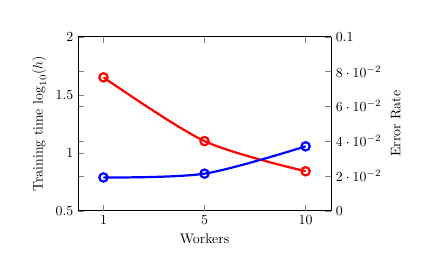
\begin{tikzpicture}[scale=0.5]
\begin{axis}[
    xmin=0, xmax=4,
  axis y line*=left,
	width=8cm, height=6cm,
  ylabel={Training time $\log_{10}(h)$},
  ymin=0.5, ymax=2,
  xlabel=Workers,
  xmin = 0.75, xmax = 3.25,
  xtick= {1,2,3},
  xticklabels={},
  extra x ticks={1,2,3},
  extra x tick style={xticklabels={1,5,10}}
  %xticklabels={0,1,5,10,15},
]
\addplot[smooth, mark=o, mark size=3pt, red, ultra thick]
coordinates{
    (1,1.65)
    (2,1.10)
    (3,0.84)
}; \label{plot_one}
%\addlegendentry{plot 1}
\end{axis}

\begin{axis}[
	width=8cm, height=6cm,
  ylabel={Error Rate},
  axis x line=none,
  xmin = 0.75, xmax = 3.25,
  ymin=0, ymax=0.1,
  ylabel near ticks, yticklabel pos=right
%% axis y line*=right
]
\addplot[smooth, mark=o, mark size=3pt, blue, ultra thick]
  coordinates{
    (1,0.0191)
    (2,0.0213)
    (3,0.037)
}; \label{plot_two}
%\addlegendimage{/pgfplots/refstyle=plot_one}\addlegendentry{plot 1}
%\addlegendimage{/pgfplots/refstyle=plot_two}\addlegendentry{plot 2}
\end{axis} 
\end{tikzpicture} 
%% &
%% \begin{tikzpicture}[scale=0.32]
%% \pgfplotsset{
%%     scale only axis,
%%     xmin=0, xmax=4
%% }

%% \begin{axis}[
%%   axis y line*=left,
%%   ylabel={Training time},
%%   ymin=6, ymax=17,
%%   xlabel=Workers,
%%   xmin = 0.75, xmax = 3.25,
%%   xtick= {1,2,3},
%%   xticklabels={},
%%   extra x ticks={1,2,3},
%%   extra x tick style={xticklabels={1,5,10}}
%%   %xticklabels={0,1,5,10,15},
%% ]
%% \addplot[smooth, mark=o, mark size=3pt, red, ultra thick]
%%   coordinates{
%%     (1,16)
%%     (2,12.6)
%%     (3,8)
%% }; \label{plot_one}
%% %\addlegendentry{plot 1}
%% \end{axis}

%% \begin{axis}[
%%   axis y line*=right,
%%   ylabel={Error Rate},
%%   axis x line=none,
%%   xmin = 0.75, xmax = 3.25,
%%   ymin=0, ymax=0.22
%% ]
%% \addplot[smooth, mark=o, mark size=3pt, blue, ultra thick]
%%   coordinates{
%%     (1,0.01)
%%     (2,0.04)
%%     (3,0.15)
%% }; \label{plot_two}
%% %\addlegendimage{/pgfplots/refstyle=plot_one}\addlegendentry{plot 1}
%% %\addlegendimage{/pgfplots/refstyle=plot_two}\addlegendentry{plot 2}
%% \end{axis} 
%% \end{tikzpicture}\\
%% \multicolumn{1}{c}{
\includegraphics[width=150pt]{figures/legend_async.pdf}
%% }
%% \end{tabular}
\end{center}
\caption{Comparison of training time and error rate for asynchronous \name{dgp-rbf} with 1, 5 and 10 workers.}
\label{fig:async}
\end{figure}


We report the results in Figure~\ref{fig:async}, and as expected, the training time decreases in proportion to the number of workers, albeit sub-linearly.
On the other hand, the increasing error rate confirms our intuition that imprecise updates of the gradients negatively impact the optimization procedure. 
The work in~\citet{Chen16} corroborates our findings, and motivates efforts in the direction of alleviating this issue.


\end{document}


\end{document}
